\documentclass[tikz,border=8pt]{standalone}
\usepackage[T1]{fontenc}
\usepackage{helvet}
\renewcommand{\familydefault}{\sfdefault}
\usetikzlibrary{arrows.meta, backgrounds}

\definecolor{queryfill}{HTML}{DFF7F3}
\definecolor{queryborder}{HTML}{1BA99C}
\definecolor{corpusfill}{HTML}{FFF4D6}
\definecolor{corpusborder}{HTML}{D9A441}
\definecolor{llmfill}{HTML}{E9EDFF}
\definecolor{llmborder}{HTML}{6979C9}
\definecolor{outfill}{HTML}{E7F6E7}
\definecolor{outborder}{HTML}{4FA64F}
\definecolor{softgray}{HTML}{F4F7FB}
\definecolor{darkline}{HTML}{333333}

\tikzset{
  card/.style={
    rectangle,
    rounded corners=5pt,
    align=center,
    draw=darkline,
    line width=0.8pt,
    minimum height=0.82cm,
    font=\small
  },
  query/.style={card, fill=queryfill, draw=queryborder, minimum width=2.05cm},
  corpus/.style={card, fill=corpusfill, draw=corpusborder, minimum width=2.25cm},
  llm/.style={card, fill=llmfill, draw=llmborder, minimum width=2.55cm, font=\small\bfseries},
  agent/.style={card, fill=llmfill, draw=llmborder, minimum width=1.7cm, font=\scriptsize\bfseries},
  output/.style={card, fill=outfill, draw=outborder, minimum width=2.6cm},
  artifact/.style={card, fill=white, minimum width=2.75cm},
  softbox/.style={rectangle, rounded corners=8pt, draw=darkline, fill=softgray, line width=0.7pt},
  doc/.style={rectangle, rounded corners=4pt, fill=corpusfill, draw=corpusborder, line width=0.7pt, minimum width=0.42cm, minimum height=0.58cm},
  node/.style={circle, fill=outfill, draw=outborder, line width=0.7pt, minimum size=0.28cm},
  phase/.style={font=\small\bfseries, align=center},
  flow/.style={-{Latex[length=2.2mm]}, line width=0.85pt, draw=darkline},
  faint/.style={dashed, darkline, opacity=0.32}
}

\begin{document}
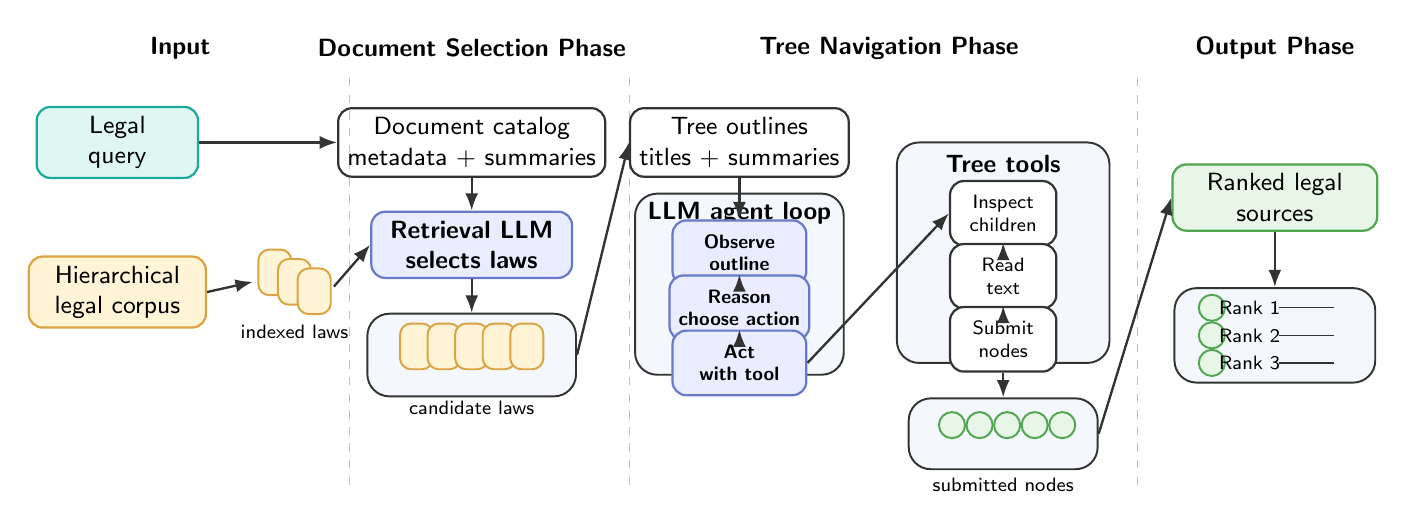
\begin{tikzpicture}

% Phase labels.
\node[phase] at (1.1,5.65) {Input};
\node[phase] at (4.8,5.65) {Document Selection Phase};
\node[phase] at (10.1,5.65) {Tree Navigation Phase};
\node[phase] at (15.0,5.65) {Output Phase};

% Input.
\node[query] (query) at (0.3,4.45) {Legal\\query};
\node[corpus] (corpus) at (0.3,2.55) {Hierarchical\\legal corpus};

% Indexed laws token stack.
\foreach \x/\y in {2.3/2.8,2.55/2.68,2.8/2.56} {
  \node[doc] at (\x,\y) {};
}
\node[font=\scriptsize] at (2.55,2.05) {indexed laws};

% Document selection.
\node[artifact] (catalog) at (4.8,4.45) {Document catalog\\metadata + summaries};
\node[llm] (selector) at (4.8,3.15) {Retrieval LLM\\selects laws};
\node[softbox, minimum width=2.65cm, minimum height=1.05cm] (lawsbox) at (4.8,1.75) {};
\foreach \x in {4.1,4.45,4.8,5.15,5.5} {
  \node[doc] at (\x,1.86) {};
}
\node[font=\scriptsize] at (4.8,1.08) {candidate laws};

% Tree navigation. Keep agent loop and tools separate to avoid overlaps.
\node[artifact] (outline) at (8.2,4.45) {Tree outlines\\titles + summaries};

\node[softbox, minimum width=2.65cm, minimum height=2.3cm] (agentbox) at (8.2,2.65) {};
\node[font=\small\bfseries] at (8.2,3.55) {LLM agent loop};
\node[agent] (observe) at (8.2,3.05) {Observe\\outline};
\node[agent] (reason) at (8.2,2.35) {Reason\\choose action};
\node[agent] (act) at (8.2,1.65) {Act\\with tool};

\node[softbox, minimum width=2.7cm, minimum height=2.8cm] (toolbox) at (11.55,3.05) {};
\node[font=\small\bfseries] at (11.55,4.18) {Tree tools};
\node[artifact, minimum width=1.35cm, font=\scriptsize] (inspect) at (11.55,3.55) {Inspect\\children};
\node[artifact, minimum width=1.35cm, font=\scriptsize] (read) at (11.55,2.75) {Read\\text};
\node[artifact, minimum width=1.35cm, font=\scriptsize] (submit) at (11.55,1.95) {Submit\\nodes};

\node[softbox, minimum width=2.4cm, minimum height=0.9cm] (submitted) at (11.55,0.75) {};
\foreach \x in {10.9,11.25,11.6,11.95,12.3} {
  \node[node] at (\x,0.86) {};
}
\node[font=\scriptsize] at (11.55,0.1) {submitted nodes};

% Output.
\node[output] (ranked) at (15.0,3.75) {Ranked legal\\sources};
\node[softbox, minimum width=2.55cm, minimum height=1.2cm] (rankbox) at (15.0,2.0) {};
\foreach \y/\lab in {2.35/1,2.0/2,1.65/3} {
  \node[node] at (14.2,\y) {};
  \node[font=\scriptsize] at (14.68,\y) {Rank \lab};
  \draw[darkline, line width=0.5pt] (15.05,\y) -- (15.75,\y);
}

% Main flow.
\draw[flow] (query.east) -- (catalog.west);
\draw[flow] (corpus.east) -- (2.02,2.68);
\draw[flow] (3.05,2.62) -- (selector.west);
\draw[flow] (catalog) -- (selector);
\draw[flow] (selector) -- (lawsbox);
\draw[flow] (lawsbox.east) -- (outline.west);
\draw[flow] (outline) -- (observe);
\draw[flow] (observe) -- (reason);
\draw[flow] (reason) -- (act);
\draw[flow] (act.east) -- (inspect.west);
\draw[flow] (inspect) -- (read);
\draw[flow] (read) -- (submit);
\draw[flow] (submit) -- (submitted);
\draw[flow] (submitted.east) -- (ranked.west);
\draw[flow] (ranked) -- (rankbox);

% Phase separators.
\draw[faint] (3.25,0.1) -- (3.25,5.35);
\draw[faint] (6.8,0.1) -- (6.8,5.35);
\draw[faint] (13.25,0.1) -- (13.25,5.35);

\end{tikzpicture}
\end{document}
